%%%% Ecriture du plan

\section*{Introduction}

\section{Etat de l'art}

\subsection{Problématiques et historique}

% idée : d'où ça sort ce concept de gestionnaire de versions ?
% Quels problèmes ont été résolus par les gestionnaires de versions, comment/quels sont les différentes solutions? 

\subsubsection{Mauvaises pratiques}

Au commencement était l'information. Et l'information était à gérer et l'information posa problème. Les développeurs de logiciels qui travaillaient en équipe devaient se soucier de mettre en commun leurs modifications. 
Nous étions à la préhistoire de l'informatique.
% (ère qui n'est peut-être pas révolue de nos jours, comme nous verrons par la suite)

Plusieurs solutions furent envisagées, des plus téméraires aux plus banales:
\begin{itemize}
\item CPOLD : pour mettre en commun une modification, nous gardions une copie du fichier d'origine, renommé en \texttt{.old} et nous copions le nouveau fichier sur un répertoire commun. 
\item La solution de la disquette : chaque modification pouvait être transmise par un nouveau fichier via une disquette, un e-mail ou autre.
\item De nos jours encore, certaines personnes utilisent un service de synchronisation dans le cloud (du type Dropbox/SugarSync) pour synchroniser leurs fichiers et dossiers sur tous les ordinateurs. 
\end{itemize}

Ces façons de gérer les ressources présentaient de nombreux défauts. Nous pouvons noter en particulier : 
\begin{enumerate}
\item le manque de robustesse et la perte de données possibles en cas d'erreur lors de la copie
\item la redondance de l'information. Une grande partie des modifications n'affecte pas l'ensemble du fichier. 
\item le manque d'automatisation. Les opérations étaient réalisées à la main -- ou au mieux à l'aide de scripts bash, MDR! 
\end{enumerate}




\begin{figure}[h!]
  \centerline{
  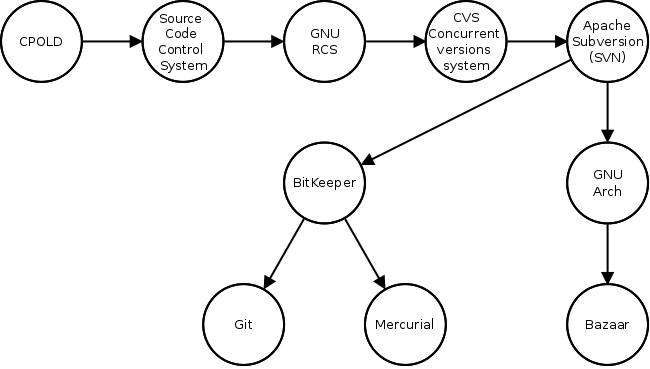
\includegraphics[width=14cm]{images/chronologie.png}}
  \caption{Résumé des gestionnaires de versions à travers l'histoire}
  \label{fig:chronologie}
\end{figure}


\subsection{Cahier des charges d'un gestionnaire de versions}

% idée : c'est quoi un gestionnaire de versions ?
% et qu'est-ce qui les distingue?

% On récapitule toutes les fonctionnalités clés : branches, commit, merge, stage, repo, centralisé, décentralisé, diff

\subsection{Récapitulatif/Comparatif des gestionnaires de versions}

% idée : quels sont les différents gestionnaires de versions ? Qu'est-ce qui les différencie ? 
% & Comment sont-ils apparus ?
% - bitkeeper, git
% - cvs, svn

\section{Etude de GIT}

\subsection{Choix de GIT}

\subsection{Utilisation de GIT}

\subsection{Détails sur le fonctionnement de GIT}

\section*{Conclusion}



%%% Local Variables: 
%%% mode: latex
%%% TeX-master: "rapport_master"
%%% End: 
